\section{Merge Reduction}\seclabel{MergeReduction}
In \secref{InvariantClosure}, we discussed how \invariantconfluence{} is
fundamentally a property of reachability and that \invariantclosure{} is
sufficient but not necessary for \invariantconfluence{} because it fails to
incorporate any notion of reachability. Using this intuition, we established
\thmref{IclosureEquivalentIconfluence} and then exploited the theorem in
\algoref{InteractiveDecisionProcedure}. In this section, we again take
advantage of this intuition to develop a new sufficient condition for
\invariantconfluence{} that can be checked without user interaction and that
covers some cases not covered by \invariantclosure{}.

An expression $e = t_1(t_2(\ldots(t_n(s))\ldots))$ is \defword{merge-free} if
does not contain any merges (i.e.\ it is generated by the grammar $e ::= s \mid
t(e)$). An object $O = (S, \join)$ is \defword{merge-reducible} with respect to
a start state $s_0 \in S$, a set of transactions $T$, and an invariant $I$,
abbreviated \defword{\sTImergereducible}, if for every pair $e_1$ and $e_2$ of
merge-free \sTIreachable{} expressions, there exists some merge-free
\sTIreachable{} expression $e_3$ that evaluates to the same state as $e_1 \join
e_2$. Intuitively, if $O$ is merge-reducible, we can replace $e_1 \join e_2$
(which has one merge) with $e_3$ (which has no merges) to obtain an equivalent
expression with fewer merges.

\begin{theorem}\thmlabel{ReducibilityImpliesIconfluence}
  Given an object $O = (S, \join)$, a start state $s_0 \in S$, a set of
  transactions $T$, and an invariant $I$, if $I(s_0)$ and if $O$ is
  \sTImergereducible{}, then $O$ is \sTIconfluent{}.
\end{theorem}

\begin{techreport}
  The proof of \thmref{ReducibilityImpliesIconfluence} is a straightforward
  induction. We begin with an \sTIreachable{} expression $e$ and repeatedly
  replace any subexpression that merges two merge-free subexpressions with an
  equivalent merge-free reachable subexpression (which we can do because $O$ is
  merge-reducible). We repeat this process until $e$ has been completely
  replaced with an equivalent merge-free reachable expression $e'$. Because
  $I(s_0)$ and because our system model only executes transactions that
  preserve the invariant, $e'$ (and hence $e$) is guaranteed to satisfy the
  invariant. Thus, all reachable states satisfy the invariant, so $O$ is
  \invariantconfluent{}.
\end{techreport}

Merge-reducibility is a sufficient condition for \invariantconfluence{}, but
unlike with \invariantclosure{}, it is not straightforward to automatically
determine if an object is merge-reducible. In \thmref{LatticeProperty}, we
outline a sufficient condition for merge-reducibility that is straightforward
to determine automatically.

\begin{theorem}\thmlabel{LatticeProperty}
  Given an object $O = (S, \join)$, a start state $s_0 \in S$, a set of
  transactions $T$, and an invariant $I$, if the following criteria are met,
  then $O$ is \sTImergereducible{} (and therefore \sTIconfluent{}).
  \begin{enumerate}
    \item
      $O$ is a join-semilattice.

    \item
      For every $t \in T$, there exists some $s_t \in S$ such that for all $s
      \in S$, $t(s) = s \join s_t$. That is, every transaction $t$ is of the
      form $t(s) = s \join s_t$ for some constant $s_t$.

    \item
      For every pair of transactions $t_1, t_2 \in T$ and for all states $s \in
      S$, if $I(s)$, $I(t_1(s))$, and $I(t_2(s))$, then $I(t_1(s) \join
      t_2(s))$.

    \item
      $I(s_0)$.
  \end{enumerate}
\end{theorem}

\begin{techreport}
  To show that $O$ is \sTImergereducible, we consider two merge-free reachable
  expressions
  \[
    e_1 = t_1(\ldots(t_n(s_0))\ldots)
    \quad\text{and}\quad
    e_2 = u_1(\ldots(u_m(s_0))\ldots)
  \]
  Then, we inductively use criterion (3) with criteria (1) and (2) to show that
  \[
    e_3 = t_1(\ldots(
    t_n(u_1(\ldots(u_m(s_0))\ldots))
    )\ldots)
  \]
  is reachable and evaluates to $e_1 \join e_2$.
\end{techreport}

\thmref{IclosureImpliesIconfluence} states that \invariantclosure{} is a
sufficient condition for \invariantconfluence{}, and \thmref{LatticeProperty}
states that criteria (1) -- (4) are sufficient conditions for
\invariantconfluence{}. How do these sufficient conditions relate to one
another?  Clearly, not all \invariantclosed{} objects are semilattices, so
\invariantclosure{} does not imply criteria (1) -- (4). Conversely, there are
some objects that satisfy criteria (1) -- (4) that are not
\invariantclosed{}. Here's one example.

\begin{example}\examplelabel{TwoSets}
  Let $O = (\mathcal{P}(\nats), \cup)$ where $\mathcal{P}(\nats)$ is the power
  set of the natural numbers. Our start state $s_0 = \set{0}$ is the set of
  $0$. Let $t_Y(X) = X \cup Y$ be the transaction that unions $Y$ with its
  argument $X$. Our set $T = \setst{t_Y}{Y \subseteq \nats}$ of transactions
  consists of all possible $t_Y$. Our invariant $I$ consists of all non-empty
  sets $X$ that contain only even or only odd elements. That is, $I = \setst{X
  \subseteq 2\nats}{X \neq \emptyset} \cup \setst{X \subseteq 2\nats + 1}{X
  \neq \emptyset}$.

  Criteria (1), (2), (3) and (4) are all satisfied. However, $O$ is not
  \Iclosed{}. Let $s_1 = \set{0}$ and $s_2 = \set{1}$. Then, $I(s_1)$ and
  $I(s_2)$, but letting $s_3 = s_1 \cup s_2 = \set{0, 1}$, $\lnot I(s_3)$.

  \begin{techreport}

    Here's why criterion (3) is satisfied. If $s$ is an arbitrary state that
    satisfies $I$, then it is non-empty and contains, without loss of generality,
    only even integers. If $t_1$ and $t_2$ are arbitrary transactions such that
    $I(t_1(s))$ and $I(t_2(s))$, then $t_1(s)$ and $t_1(s)$ are also non-empty
    and contain only even integers. Thus, $t_1(s) \cup t_2(s)$ is clearly
    non-empty and contains only even integers, so $I(t_1(s) \join t_2(s))$.
  \end{techreport}
\end{example}

% {\begin{figure}[t]
  \centering
  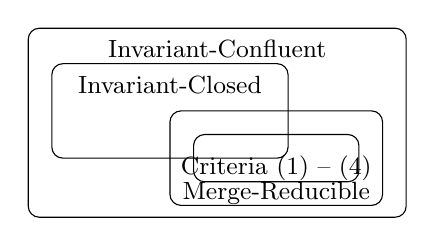
\begin{tikzpicture}[scale=0.3]
    \draw[rounded corners] (0, 0) rectangle (16, 8);
    \draw[rounded corners] (1, 2.5) rectangle (11, 6.5);
    \draw[rounded corners] (6, 0.5) rectangle (15, 4.5);
    \draw[rounded corners] (7, 1.5) rectangle ++(7, 2);
    \node[inner sep=0pt, anchor=north] at (8, 7.5) {\small Invariant-Confluent};
    \node[inner sep=0pt, anchor=north] at (6, 6) {\small Invariant-Closed};
    \node[inner sep=0pt, anchor=south] at (10.5, 1.5) {\small Criteria (1) -- (4)};
    \node[inner sep=0pt, anchor=south] at (10.5, 0.5) {\small Merge-Reducible};
  \end{tikzpicture}
  \caption{%
    The relationship between invariant-closure, merge-reducibility, criteria
    (1) -- (4) from \thmref{LatticeProperty}, and invariant-confluence.
  }\figlabel{IclosureVsReducible}
\end{figure}
}

\Invariantclosure{} is not necessary for \invariantconfluence{} because it
fails to incorporate any notion of reachability. Criteria (1) -- (4) are also
unnecessary, but they can be used to prove that some non-\invariantclosed{}
objects are \invariantconfluent{} because the criteria \emph{do} incorporate
notions of reachability. In particular, criterion (3) is a slight variant of
\invariantclosure{}; it also states that invariant satisfying states should be
closed under merge. The fundamental difference is that criterion (3) restricts
its attention to the merge of two states that are \emph{reachable} from a
common ancestor state.

In \exampleref{TwoSets}, we saw this fundamental difference rear its head. $O$
is not $I$-closed because the union of an odd-only set with an even-only set is
a set with both odd and even integers. However, if we begin in an invariant
satisfying state, we cannot reach both an odd-only and even-only set.
Criterion (3) is able to recognize this fact and conclude that $O$ is
\invariantconfluent{} despite it not being \invariantclosed{}.
